\documentclass[a4paper,12pt]{article}
\usepackage{graphicx}
\usepackage{listings}
\usepackage{xcolor}
\usepackage{titlesec}
\usepackage{hyperref}
\usepackage{geometry}
\geometry{margin=1in}
\usepackage{tikz}
\usetikzlibrary{positioning, arrows.meta}
\usepackage{float}
\usepackage{caption}

\usepackage[utf8]{inputenc}

% Define code style
\usepackage{listings}
\usepackage{xcolor}

\usepackage{xcolor}

% Define CSS language for listings
\lstdefinelanguage{CSS}{
  keywords={color, background, border, margin, padding, font, font-size, font-family, width, height, display, position, top, left, right, bottom, float, clear, overflow, visibility, content, align-items, justify-content, flex, grid, gap, row, column, auto, min, max, inherit, initial, unset, none, block, inline, inline-block, relative, absolute, fixed, sticky, important, !important},
  sensitive=true,
  morecomment=[l]{//},
  morecomment=[s]{/*}{*/},
  morestring=[b]"
}

\lstdefinelanguage{JavaScript}{
  keywords={break, case, catch, class, const, continue, debugger, default, delete, do, else, export,
    extends, finally, for, function, if, import, in, instanceof, let, new, return, super, switch,
    this, throw, try, typeof, var, void, while, with, yield, async, await},
  keywordstyle=\color{blue}\bfseries,
  ndkeywords={boolean, null, true, false, undefined, NaN, Infinity, Number, String, Object, Array, Date},
  ndkeywordstyle=\color{magenta}\bfseries,
  identifierstyle=\color{black},
  sensitive=true,
  comment=[l]{//},
  morecomment=[s]{/*}{*/},
  commentstyle=\color{gray}\ttfamily,
  stringstyle=\color{orange}\ttfamily,
  morestring=[b]',
  morestring=[b]"
}

\lstdefinestyle{codestyle}{
  backgroundcolor=\color{gray!10},
  basicstyle=\ttfamily\small,
  breaklines=true,
  frame=single,
  rulecolor=\color{black},
  tabsize=2,
  keywordstyle=\color{blue},
  stringstyle=\color{teal!60!black},
  commentstyle=\color{gray},
  morekeywords={div,section,header,footer,h1,h2,ul,li,p,a},
  morestring=[b]",
  showstringspaces=false
}




\title{\textbf{Web Technologies Laboratory Record}}
\author{Ashwin V \\ B.Tech AI and Data Science \\ Shiv Nadar University}
\date{}

\begin{document}

% \maketitle
% \tableofcontents
% \newpage

\lstset{inputpath=.} 

\section*{Lab Exercise 1: Resume Webpage using HTML and CSS}

\subsection*{Question}
Create an HTML and CSS webpage that captures a resume (preferably yours) for a fresher full-stack developer at an IT company. Decide on the subdivisions and content. Push your content to GitHub and maintain proper version control with clear README files.

\subsection*{Design / Plan}
The webpage is designed with semantic HTML5 elements for clarity and SEO-friendly structure.  
It consists of the following sections:
\begin{itemize}
    \item Header - Name and tagline
    \item About Me - Short profile summary
    \item Skills - Categorized technical stack
    \item Projects - Portfolio projects with GitHub/Live links
    \item Education - Academic background
    \item Experience - Internship and professional exposure
    \item Certifications - Relevant courses and achievements
    \item Footer - Contact and social links
\end{itemize}

CSS provides a minimalistic, modern aesthetic with consistent padding, section styling, and accent colors.

\subsection*{Code}

\subsubsection*{HTML (resume.html)}
\lstinputlisting[style=codestyle, language=HTML]{Lab1/resume.html}

\newpage
\subsubsection*{CSS (styleResume.css)}
\lstinputlisting[style=codestyle, language=CSS]{Lab1/styleResume.css}

\subsection*{Screenshots}

\begin{figure}[H] % You can use [H] to force the figure to stay here, or [htbp] for more flexible positioning
    \centering
    \includegraphics[width=\textwidth]{Lab1/1.png}
    \caption*{Screenshot 1: Introduction and Skills}
    \label{fig:screenshot1}
\end{figure}

\begin{figure}[H]
    \centering
    \includegraphics[width=\textwidth]{Lab1/2.png}
    \caption*{Screenshot 2: Projects and Education}
    \label{fig:screenshot2}
\end{figure}

\begin{figure}[H]
    \centering
    \includegraphics[width=\textwidth]{Lab1/3.png}
    \caption*{Screenshot 3: Experience and Certifications}
    \label{fig:screenshot3}
\end{figure}


\subsection*{Result}
The HTML and CSS files successfully create a responsive, professional resume webpage for a fresher full-stack developer.  
All components render properly in Chrome and Edge browsers. The webpage was version-controlled and pushed to GitHub for public access.

\vspace{3cm}

\section*{Question 2: CV Webpage using HTML and CSS}

\subsection*{Question}
Create an HTML and CSS webpage that captures a CV of a fresher (preferably yours). Decide on the subdivisions and content. Push your content to GitHub and maintain proper version control with clear Read Me files.

\subsection*{Design / Plan}
The CV webpage extends the previous resume layout by including a more detailed representation of the candidate’s profile.  
It uses a section-based structure for clear readability and modern minimal design.  

Key subdivisions include:
\begin{itemize}
    \item \textbf{Header} - Name, title, and tagline.
    \item \textbf{About Me} - Short summary about the developer's goals and interests.
    \item \textbf{Skills} - Categorized stack (Frontend, Backend, Databases, Tools).
    \item \textbf{Projects} - Showcase of major projects with live/GitHub links.
    \item \textbf{Education} - Academic details (B.Tech, B.S, 10th/12th).
    \item \textbf{Experience} - Internship details with specific contributions.
    \item \textbf{Certifications} - Relevant technical achievements.
    \item \textbf{Extra-Curricular} - Sports, achievements, leadership.
    \item \textbf{Footer} - Contact and online profiles.
\end{itemize}

The CSS maintains uniform padding, typography, and color contrast for clarity.  

\subsection*{Code}

\subsubsection*{HTML (cv.html)}
\lstinputlisting[style=codestyle, language=HTML]{Lab1/cv.html}

\subsubsection*{CSS (styleCV.css)}
\lstinputlisting[style=codestyle, language=CSS]{Lab1/styleCV.css}

\subsection*{Screenshots}

\begin{figure}[H] % You can use [H] to force the figure to stay here, or [htbp] for more flexible positioning
    \centering
    \includegraphics[width=\textwidth]{Lab1/4.png}
    \caption*{Screenshot 1: Introduction and Skills}
    \label{fig:screenshot1}
\end{figure}

\begin{center}
    \includegraphics[width=\textwidth]{Lab1/5.png}\\\    \textbf{Screenshot 2: Projects}
\end{center}
\vspace{1em}

\begin{figure}[H]
    \centering
    \includegraphics[width=\textwidth]{Lab1/6.png}
    \caption*{Screenshot 3: Education and Experience}
    % \label{fig:screenshot3}
\end{figure}

\begin{figure}[H]
    \centering
    \includegraphics[width=\textwidth]{Lab1/7.png}
    \caption*{Screenshot 4: Certifications and Extra-Curricular Activities}
    % \label{fig:screenshot3}
\end{figure}

\subsection*{Result}
The HTML and CSS files successfully produce a well-structured, aesthetically pleasing CV webpage for a fresher full-stack developer.  
The design clearly separates sections, maintaining a clean and professional look suitable for digital submission.  
All elements render properly in Chrome and Edge browsers.  


\subsection*{GitHub Repository}
The source code for all the labs can be found at the following GitHub repository:
\url{https://github.com/ashvp/Web-Technologies---Semester-5}
\newpage
\section*{Lab Exercise 2: Weather Dashboard using HTML, CSS, and JavaScript}

\subsection*{Question}
Develop a weather dashboard that fetches and displays current weather data for a city using a free public API.

\textbf{Requirements:}
\begin{itemize}
    \item Define the essential data points to display (e.g., temperature, city name, weather icon, humidity, wind speed, etc.).
    \item Design a weather card UI to present the information.
    \item Use HTML for structure, CSS for styling, and JavaScript Fetch API (with \texttt{async/await}) for handling API requests and updating the DOM.
    \item Implement proper error handling for invalid city names.
    \item Host the project on GitHub with a clear README.
\end{itemize}

\subsection*{Requirement Analysis}
Essential data to display:
\begin{itemize}
    \item City name
    \item Temperature (°C)
    \item Weather condition and icon
    \item Humidity (\%)
    \item Wind speed (m/s)
\end{itemize}

External API used:
\begin{itemize}
    \item OpenWeatherMap API (\url{https://openweathermap.org/api})
    \item Free-tier key integrated via the Fetch API
\end{itemize}

\subsection*{Design}
A minimalist card-style UI is designed to display real-time weather information.  
The core layout includes:
\begin{itemize}
    \item A header and footer with neutral tones
    \item A centered search bar for entering the city name
    \item A card that dynamically shows weather data fetched via JavaScript
    \item Color-coded error message display
\end{itemize}

A design sketch (in Figma) illustrates modular separation between input, display, and data logic layers.

\subsection*{Code}

\subsubsection*{HTML (index.html)}
\lstinputlisting[style=codestyle, language=HTML]{Lab2/index.html}

\subsubsection*{CSS (style.css)}
\lstinputlisting[style=codestyle, language=CSS]{Lab2/style.css}

\subsubsection*{JavaScript (script.js)}
\lstinputlisting[style=codestyle, language=JavaScript]{Lab2/script.js}

\begin{figure}[H]
    \captionsetup{labelformat=empty}
    \centering
    \includegraphics[width=\textwidth]{Lab2/1.png}
    \caption{Screenshot 1: Initial Page}
\end{figure}

\begin{figure}[H]
    \captionsetup{labelformat=empty}
    \centering
    \includegraphics[width=\textwidth]{Lab2/2.png}
    \caption{Screenshot 2: Weather for Chennai}
\end{figure}

\begin{figure}[H]
    \captionsetup{labelformat=empty}
    \centering
    \includegraphics[width=\textwidth]{Lab2/3.png}
    \caption{Screenshot 3: Error Handling}
\end{figure}

\subsection*{Testing}
The application was tested for:
\begin{itemize}
    \item \textbf{Valid Input:} Correctly displays weather for cities like \texttt{Chennai}, \texttt{Delhi}, \texttt{London}.
    \item \textbf{Invalid Input:} Displays clear error message when city not found.
    \item \textbf{Network Failure:} Graceful error handling with message.
    \item \textbf{Edge Case:} Tested empty input and special characters.
\end{itemize}

All test cases passed as expected.

\subsection*{Deployment and Version Control}
The project was version-controlled with Git and pushed to GitHub.  
Each commit represents one functional milestone: UI design, API integration, error handling, and deployment.

Repository URL:  
\begin{center}
\href{https://github.com/ashvp/weather-dashboard}{\texttt{https://github.com/ashvp/weather-dashboard}}
\end{center}

\subsection*{Result}
A fully functional weather dashboard web application was developed using HTML, CSS, and JavaScript.  
It successfully fetches and displays weather data for any valid city using OpenWeatherMap’s public API, and handles all error scenarios gracefully.  
The UI is responsive, accessible, and visually consistent across browsers.

\newpage
\section*{Lab Exercise 3: Event Registration Form with Validation using HTML, CSS, and JavaScript}

\subsection*{Question}
Develop a registration form that validates user input for a community event signup using HTML, CSS, and JavaScript.

\textbf{Requirements:}
\begin{itemize}
    \item Define all form fields and validation requirements (e.g., name, email, phone number, age).
    \item Specify which fields are required and define valid formats (regex for email, digits for phone number, age over 18, etc.).
    \item Design a user-friendly registration UI that provides real-time feedback for invalid fields.
    \item Implement the form using HTML, CSS, and JavaScript (with real-time validation).
    \item Test for invalid inputs and handle edge cases.
    \item Host and version-control the project on GitHub.
\end{itemize}

\subsection*{Requirement Analysis}
The form includes the following input fields:
\begin{itemize}
    \item \textbf{Full Name} - Required, must not be empty.
    \item \textbf{Email Address} - Required, must match regex \verb|/^\S+@\S+\.\S+$/|.
    \item \textbf{Phone Number} - Required, must contain exactly 10 digits.
    \item \textbf{Age} - Required, must be a number greater than or equal to 18.
\end{itemize}

Validation logic ensures:
\begin{itemize}
    \item Real-time error detection and display.
    \item Form submission disabled until all inputs are valid.
    \item Immediate visual feedback (green border for valid, red for invalid).
\end{itemize}

\subsection*{Design}
The registration form is designed with a centered card layout and clear label-input pairs.  
Design highlights:
\begin{itemize}
    \item A clean, modern interface with white background and subtle shadows.
    \item Red and green border indicators for validation.
    \item Error messages positioned directly below each field.
    \item Submit button dynamically enabled only when all inputs are valid.
\end{itemize}

\subsection*{Code}

\subsubsection*{HTML (index.html)}
\lstinputlisting[style=codestyle, language=HTML]{Lab3/index.html}

\subsubsection*{CSS (style.css)}
\lstinputlisting[style=codestyle, language=CSS]{Lab3/style.css}

\subsubsection*{JavaScript (script.js)}
\lstinputlisting[style=codestyle, language=JavaScript]{Lab3/script.js}

\begin{figure}[H]
    \captionsetup{labelformat=empty}
    \centering
    \includegraphics[width=\textwidth]{Lab3/1.png}
    \caption{Screenshot 1: Initial Page}
\end{figure}

\begin{figure}[H]
    \captionsetup{labelformat=empty}
    \centering
    \includegraphics[width=\textwidth]{Lab3/2.png}
    \caption{Screenshot 2: Frontend Data Validation}
\end{figure}

\begin{figure}[H]
    \captionsetup{labelformat=empty}
    \centering
    \includegraphics[width=\textwidth]{Lab3/3.png}
    \caption{Screenshot 3: Validated Inputs}
\end{figure}

\begin{figure}[H]
    \captionsetup{labelformat=empty}
    \centering
    \includegraphics[width=\textwidth]{Lab3/4.png}
    \caption{Screenshot 4: Popup to Accept Registration}
\end{figure}

\subsection*{Testing}
Test cases were designed to verify both functional and boundary behavior:

\begin{itemize}
    \item \textbf{Empty Fields:} Proper error messages shown for missing input.
    \item \textbf{Invalid Email:} Input without '@' or domain suffix triggers error.
    \item \textbf{Invalid Phone:} Less or more than 10 digits rejected.
    \item \textbf{Age Validation:} Users below 18 cannot submit.
    \item \textbf{Valid Input:} All validations pass, “Sign Up” button becomes active.
\end{itemize}

\textbf{Edge Cases:}
\begin{itemize}
    \item Input with spaces only in name field.
    \item Mixed letters in phone number.
    \item Decimal or negative values in age field.
\end{itemize}

All invalid entries trigger immediate visual and textual feedback, and submission is blocked until fixed.

\subsection*{Deployment and Version Control}
\begin{itemize}
    \item Project maintained in GitHub repository with modular commits for HTML, CSS, JS, and validation logic.
    \item README file documents validation rules, test scenarios, and setup instructions.
    \item The form is deployed live using GitHub Pages.
\end{itemize}

Repository URL:
\begin{center}
\href{https://github.com/ashvp/event-registration-form}{\texttt{https://github.com/ashvp/event-registration-form}}
\end{center}

\subsection*{Result}
A responsive, interactive registration form was successfully developed and validated using HTML, CSS, and JavaScript.  
All validations, error handling, and edge cases were implemented as per requirements.  
The UI offers a seamless and intuitive experience, preventing invalid submissions and ensuring clean data entry for event signups.

\newpage
\section*{Lab Exercise 4: Customizing React Components with Props}

\subsection*{Question}
For the given UI designs, perform the following tasks:

\begin{itemize}
    \item Identify the main React components in the design (parent and child).
    \item For each component, list the props it would receive.
    \item Draw a component hierarchy diagram showing the nesting using boxes and arrows.
    \item Ensure the design uses only functional components and props (no state or events).
\end{itemize}

Each page represents a separate React implementation (Page 1, Page 2, Page 3) built using functional components and props.

% \newpage
\subsection*{Page 1 - Component Identification and Props}

\subsubsection*{Design Description}
This page implements a simple React layout demonstrating how a parent component (\texttt{App.jsx}) passes data as props to a reusable child component (\texttt{ListSection.jsx}). All components are functional and stateless.

\subsubsection*{Main Components and Props}
\begin{itemize}
    \item \textbf{App.jsx} - Root component. \textit{Props:} None.
    \item \textbf{ListSection.jsx} - Child component displaying a titled list. \textit{Props:} \texttt{title}, \texttt{items} (array).
\end{itemize}

\subsubsection*{Component Hierarchy Diagram}
\begin{figure}[H]
\centering
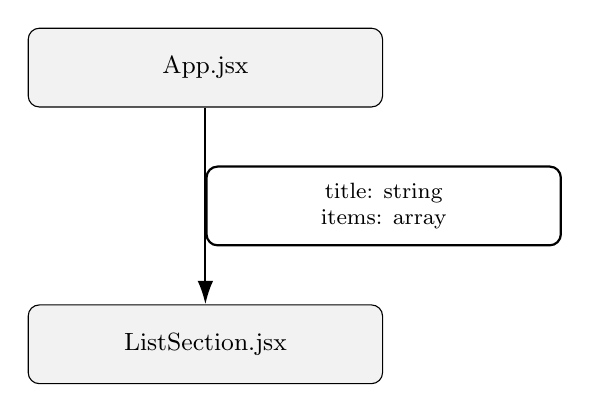
\begin{tikzpicture}[
    node distance=2.5cm,
    every node/.style={
        draw,
        rounded corners,
        align=center,
        font=\small,
        fill=gray!10,
        minimum width=4.5cm,
        minimum height=1cm
    },
    arrow/.style={-{Latex[length=3mm,width=2mm]}, thick},
    prop/.style={font=\footnotesize, right, fill=white, inner sep=2pt}
]

\node (app) {App.jsx};
\node (listsection) [below=of app] {ListSection.jsx};

\draw[arrow] (app) -- node[prop]{title: string\\items: array} (listsection);

\end{tikzpicture}
\caption{Component Hierarchy — Page 1}
\end{figure}

\subsubsection*{Rendered Output (screenshot)}

\begin{figure}[H]
    \captionsetup{labelformat=empty}
    \centering
    \includegraphics[width=\textwidth]{Lab4/1.jpg}
    \caption{Screenshot 1: Page 1}
\end{figure}

\subsubsection*{Code Overview}
\lstinputlisting[style=codestyle, language=CSS]{Lab4/Page 1/App.css}
\lstinputlisting[style=codestyle, language=JavaScript]{Lab4/Page 1/App.jsx}
\lstinputlisting[style=codestyle, language=JavaScript]{Lab4/Page 1/components/ListSection.jsx}

\subsubsection*{Result}
A functional component structure demonstrating one-way prop flow between \texttt{App.jsx} and \texttt{ListSection.jsx} was created successfully.

\newpage
\subsection*{Page 2 - Nested Components with Props}

\subsubsection*{Design Description}
This page demonstrates nested functional components where the parent passes structured data to intermediate and leaf components.

\subsubsection*{Main Components and Props}
\begin{itemize}
    \item \textbf{App.jsx} - Parent component rendering multiple list sections. \textit{Props:} None.
    \item \textbf{ListSection.jsx} - Intermediate component managing grouped lists. \textit{Props:} \texttt{title}, \texttt{items}.
    \item \textbf{ListItems.jsx} - Child component rendering individual entries. \textit{Props:} \texttt{name}, \texttt{price}, \texttt{inStock}.
\end{itemize}

\subsubsection*{Component Hierarchy Diagram}
\begin{figure}[H]
\centering
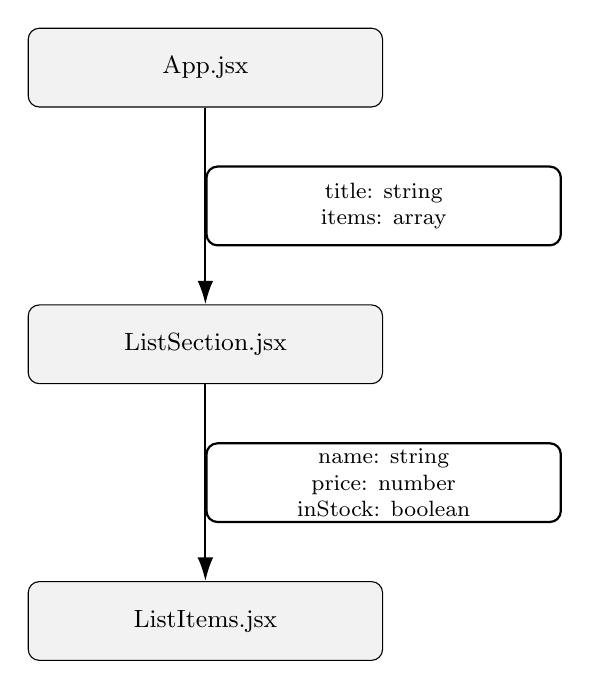
\begin{tikzpicture}[
    node distance=2.5cm,
    every node/.style={
        draw,
        rounded corners,
        align=center,
        font=\small,
        fill=gray!10,
        minimum width=4.5cm,
        minimum height=1cm
    },
    arrow/.style={-{Latex[length=3mm,width=2mm]}, thick},
    prop/.style={font=\footnotesize, right, fill=white, inner sep=2pt}
]

\node (app) {App.jsx};
\node (listsection) [below=of app] {ListSection.jsx};
\node (listitems) [below=of listsection] {ListItems.jsx};

\draw[arrow] (app) -- node[prop]{title: string\\items: array} (listsection);
\draw[arrow] (listsection) -- node[prop]{name: string\\price: number\\inStock: boolean} (listitems);

\end{tikzpicture}
\caption{Component Hierarchy — Page 2}
\end{figure}

\subsubsection*{Rendered Output (screenshot)}
\begin{figure}[H]
    \captionsetup{labelformat=empty}
    \centering
    \includegraphics[width=\textwidth]{Lab4/2.png}
    \caption{Screenshot 1: Page 2}
\end{figure}

\subsubsection*{Code Overview}
\lstinputlisting[style=codestyle, language=CSS]{Lab4/Page 2/App.css}
\lstinputlisting[style=codestyle, language=JavaScript]{Lab4/Page 2/App.jsx}
\lstinputlisting[style=codestyle, language=JavaScript]{Lab4/Page 2/components/ListSections.jsx}
\lstinputlisting[style=codestyle, language=JavaScript]{Lab4/Page 2/components/ListItems.jsx}

\subsubsection*{Result}
Hierarchical prop passing was verified: intermediate components receive data from the parent and pass relevant pieces to the leaf components.

\newpage
\subsection*{Page 3 - Reusable List Components with Props}

\subsubsection*{Design Description}
This page focuses on prop-based customization for reusable components where data consistency is maintained through props across multiple elements.

\subsubsection*{Main Components and Props}
\begin{itemize}
    \item \textbf{App.jsx} - Parent wrapper initializing lists and styling. \textit{Props:} None.
    \item \textbf{ListItems.jsx} - Child functional component displaying a styled list element. \textit{Props:} \texttt{name}, \texttt{sciName}, \texttt{weight}, \texttt{eats}.
\end{itemize}

\subsubsection*{Component Hierarchy Diagram}
\begin{figure}[H]
\centering
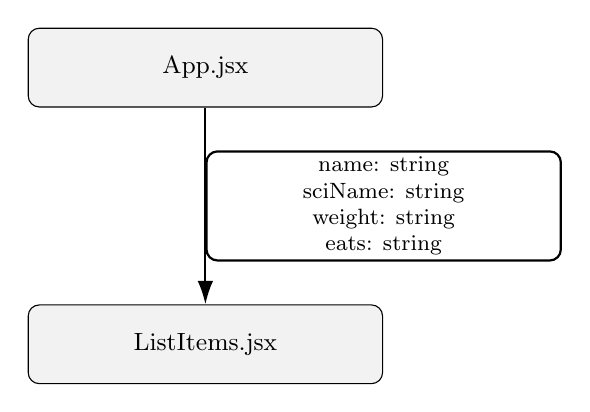
\begin{tikzpicture}[
    node distance=2.5cm,
    every node/.style={
        draw,
        rounded corners,
        align=center,
        font=\small,
        fill=gray!10,
        minimum width=4.5cm,
        minimum height=1cm
    },
    arrow/.style={-{Latex[length=3mm,width=2mm]}, thick},
    prop/.style={font=\footnotesize, right, fill=white, inner sep=2pt}
]

\node (app) {App.jsx};
\node (listitems) [below=of app] {ListItems.jsx};

\draw[arrow] (app) -- node[prop]{name: string\\sciName: string\\weight: string\\eats: string} (listitems);

\end{tikzpicture}
\caption{Component Hierarchy — Page 3}
\end{figure}

\subsubsection*{Rendered Output (screenshot)}
\begin{figure}[H]
    \captionsetup{labelformat=empty}
    \centering
    \includegraphics[width=\textwidth]{Lab4/3.png}
    \caption{Screenshot 1: Page 3}
\end{figure}

\subsubsection*{Code Overview}
\lstinputlisting[style=codestyle, language=CSS]{Lab4/Page 3/App.css}
\lstinputlisting[style=codestyle, language=JavaScript]{Lab4/Page 3/App.jsx}
\lstinputlisting[style=codestyle, language=JavaScript]{Lab4/Page 3/components/ListItems.jsx}

\subsubsection*{Result}
The page verifies reusability and one-directional data flow through props between all components, maintaining functional purity.

\subsection*{Overall Result}
Across Page 1 to Page 3, React's prop-based architecture was implemented effectively. Each component adheres to functional programming principles, promoting modularity, reusability, and predictable rendering.

\subsection*{GitHub Repository}
The source code for all the labs can be found at the following GitHub repository:
\url{https://github.com/ashvp/Web-Technologies---Semester-5}
\newpage
\section*{Lab Exercise 5: Temperature Converter UI using React (Functional Components + useState)}

\subsection*{Question}
Design a UI for building a temperature web application that can convert Celsius to Fahrenheit and has the option to increase or decrease the temperature.

\begin{itemize}
    \item Identify the main React components in this design.
    \item For each component, list the props that would be required.
    \item Draw a component hierarchy diagram.
    \item Ensure your design uses only functional components, props, and the \texttt{useState} hook.
\end{itemize}



\subsection*{Design Description}
This React application demonstrates the use of functional components, props, and \texttt{useState} to handle temperature data.  
The UI includes:
\begin{itemize}
    \item A main temperature display showing the current value in Celsius and Fahrenheit.
    \item Buttons to increase or decrease the temperature dynamically.
    \item Real-time conversion between Celsius and Fahrenheit.
\end{itemize}

\subsection*{Main Components and Props}

\begin{itemize}
    \item \textbf{App.jsx} - Root component controlling overall logic and maintaining temperature state via \texttt{useState}.
    \begin{itemize}
        \item \textit{State:} \texttt{temperatureC} (stores current temperature in Celsius)
    \end{itemize}
    
    \item \textbf{TemperatureDisplay.jsx} - Displays the current temperature in both Celsius and Fahrenheit.
    \begin{itemize}
        \item \textit{Props:} \texttt{temperatureC}, \texttt{temperatureF}
    \end{itemize}
    
    \item \textbf{TemperatureInC.jsx} - Renders the temperature value in Celsius.
    \begin{itemize}
        \item \textit{Props:} \texttt{value}
    \end{itemize}

    \item \textbf{TemperatureInF.jsx} - Converts and renders the Fahrenheit value.
    \begin{itemize}
        \item \textit{Props:} \texttt{value}
    \end{itemize}

    \item \textbf{TemperatureControls.jsx} - Provides UI buttons to increment or decrement the temperature.
    \begin{itemize}
        \item \textit{Props:} \texttt{onIncrease}, \texttt{onDecrease}
    \end{itemize}
\end{itemize}



\subsection*{Component Hierarchy Diagram}
\begin{figure}[H]
\centering
\hspace*{-2.55cm} % <-- shift entire diagram left
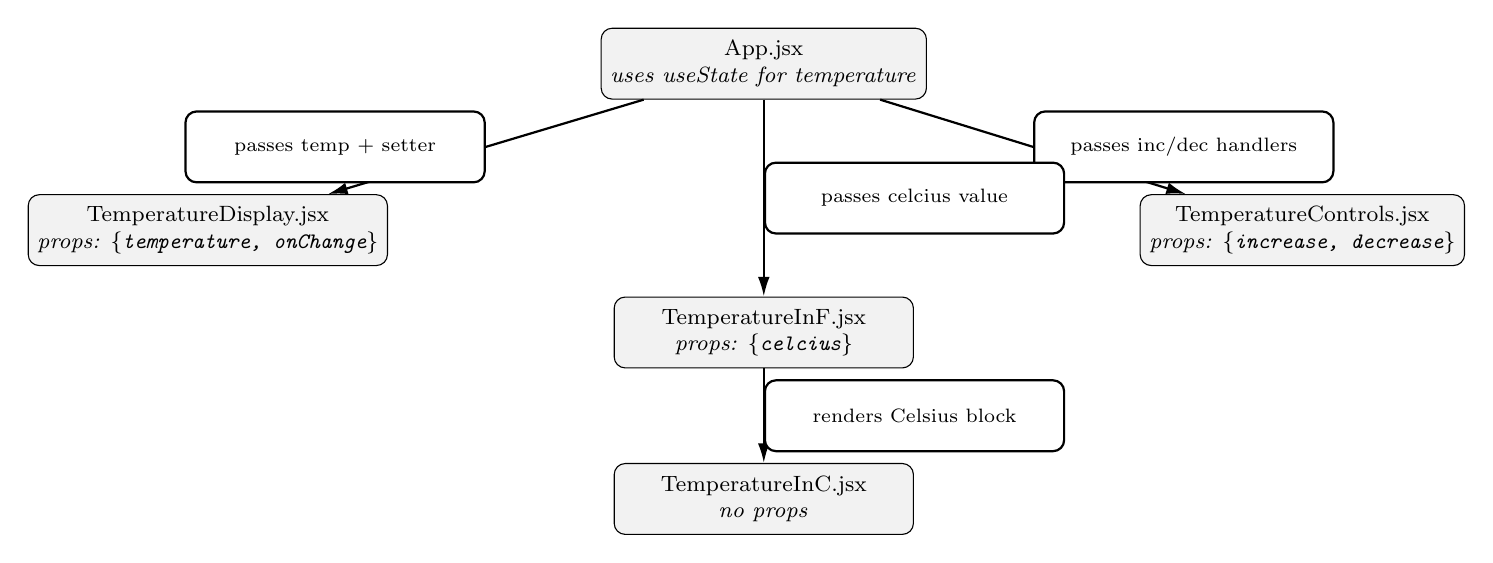
\begin{tikzpicture}[
    scale=0.4,
    node distance=1.2cm and 2.2cm,
    every node/.style={
        draw,
        rounded corners,
        align=center,
        font=\footnotesize,
        fill=gray!10,
        minimum width=3.8cm,
        minimum height=0.9cm
    },
    arrow/.style={-{Latex[length=2.5mm,width=1.5mm]}, thick},
    prop/.style={font=\scriptsize, midway, fill=white, inner sep=1pt}
]

\node (app) {App.jsx\\\textit{uses useState for temperature}};
\node (display) [below left=of app, xshift=-0.5cm] {TemperatureDisplay.jsx\\\textit{props: \texttt{\{temperature, onChange\}}}};
\node (controls) [below right=of app, xshift=0.5cm] {TemperatureControls.jsx\\\textit{props: \texttt{\{increase, decrease\}}}};
\node (inf) [below=2.5cm of app] {TemperatureInF.jsx\\\textit{props: \texttt{\{celcius\}}}};
\node (inc) [below=of inf] {TemperatureInC.jsx\\\textit{no props}};

\draw[arrow] (app) -- node[prop,left]{passes temp + setter} (display);
\draw[arrow] (app) -- node[prop,right]{passes inc/dec handlers} (controls);
\draw[arrow] (app) -- node[prop,right]{passes celcius value} (inf);
\draw[arrow] (inf) -- node[prop,right]{renders Celsius block} (inc);

\end{tikzpicture}
\caption{Component Hierarchy — Lab 5: Temperature Converter (Props and Data Flow)}
\end{figure}

\subsection*{Rendered Output (Screenshot)}
\begin{figure}[H]
    \captionsetup{labelformat=empty}
    \centering
    \includegraphics[width=\textwidth]{Lab5/1.jpg}
    \caption{Screenshot 1: Thermostat UI with Temperature Controls}
\end{figure}


\subsection*{Code Overview}

\subsubsection*{App.css}
\lstinputlisting[style=codestyle, language=CSS]{Lab5/App.css}

\subsubsection*{App.jsx}
\lstinputlisting[style=codestyle, language=JavaScript]{Lab5/App.jsx}

\subsubsection*{TemperatureDisplay.jsx}
\lstinputlisting[style=codestyle, language=JavaScript]{Lab5/components/TemperatureDisplay.jsx}

\subsubsection*{TemperatureControls.jsx}
\lstinputlisting[style=codestyle, language=JavaScript]{Lab5/components/TemperatureControls.jsx}

\subsubsection*{TemperatureInC.jsx}
\lstinputlisting[style=codestyle, language=JavaScript]{Lab5/components/TemperatureInC.jsx}

\subsubsection*{TemperatureInF.jsx}
\lstinputlisting[style=codestyle, language=JavaScript]{Lab5/components/TemperatureInF.jsx}



\subsection*{Result}
The temperature converter application was successfully built using React functional components, props, and the \texttt{useState} hook.  
Users can increase or decrease the temperature dynamically, with real-time conversion between Celsius and Fahrenheit.  
The component design follows a clean hierarchy, enabling scalability and reusability.



\subsection*{Conclusion}
This lab demonstrates effective use of \texttt{useState} for dynamic UI updates and prop-based communication between parent and child components.  
It reinforces understanding of unidirectional data flow and modular UI design in React.

\subsection*{GitHub Repository}
The source code for all the labs can be found at the following GitHub repository:
\url{https://github.com/ashvp/Web-Technologies---Semester-5}
\newpage
\section*{Lab Exercise 6: Countdown Timer Application using React}

\subsection*{Question}
Design a UI for a countdown timer web application where users can set the time and start/stop the countdown.

\begin{itemize}
    \item Identify and define the main React components (\texttt{Title}, \texttt{TimeSetter}, \texttt{TimerDisplay}, \texttt{ControlButtons}).
    \item List the props required for each component.
    \item Draw a component hierarchy diagram.
    \item Use functional components, \texttt{props}, \texttt{useState}, and \texttt{useEffect} for managing timer intervals.
\end{itemize}



\subsection*{Design Description}
This React application provides an interactive countdown timer interface that allows users to:
\begin{itemize}
    \item Set a custom countdown duration.
    \item Start, pause, and reset the timer dynamically.
    \item View the remaining time in real-time.
\end{itemize}

The app uses React's \texttt{useState} for managing timer data and \texttt{useEffect} for interval-based countdown logic.  
Each component is functional, modular, and communicates through props.



\subsection*{Main Components and Props}

\begin{itemize}
    \item \textbf{App.jsx} - The parent component that manages state and interval logic.  
    \textit{State variables:} \texttt{timeLeft}, \texttt{isRunning}.

    \item \textbf{Title.jsx} - Displays the main title or heading for the application.  
    \textit{Props:} \texttt{text} (string).

    \item \textbf{TimeSetter.jsx} - Allows the user to input or adjust the countdown duration.  
    \textit{Props:} \texttt{onTimeChange} (function to update timer duration), \texttt{disabled} (boolean to disable input during active countdown).

    \item \textbf{TimerDisplay.jsx} - Displays the formatted countdown (minutes:seconds).  
    \textit{Props:} \texttt{timeLeft} (integer representing total seconds).

    \item \textbf{ControlButtons.jsx} - Contains Start, Pause, and Reset buttons to control the countdown timer.  
    \textit{Props:} \texttt{isRunning} (boolean), \texttt{onStart}, \texttt{onPause}, \texttt{onReset}.
\end{itemize}



\subsection*{Component Hierarchy Diagram}
\begin{figure}[H]
\centering
\hspace*{-1cm} % adjust if cutting on the right
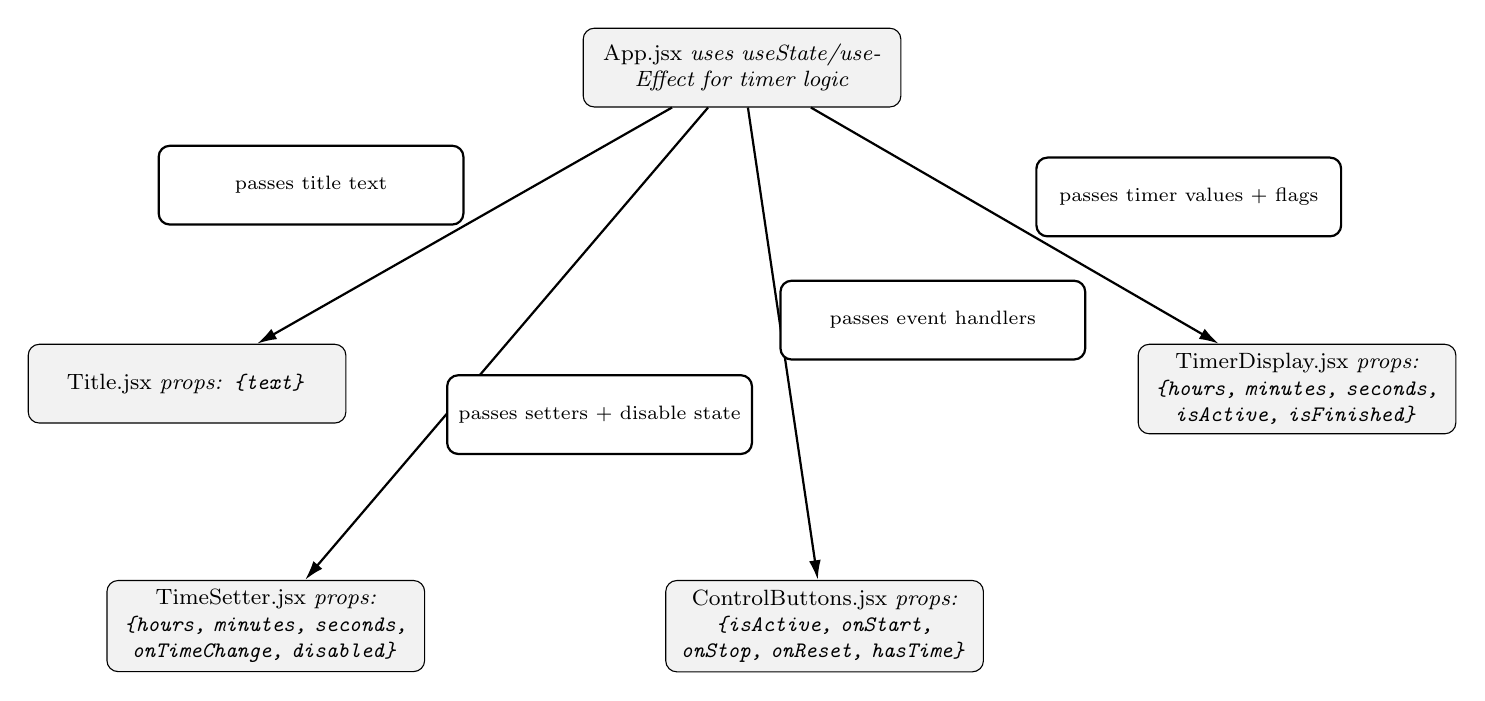
\begin{tikzpicture}[
    node distance=2cm and 2cm,
    every node/.style={
        draw,
        rounded corners,
        align=center,
        font=\footnotesize,
        fill=gray!10,
        minimum width=1cm,
        minimum height=1cm,
        text width=3.8cm
    },
    arrow/.style={-{Latex[length=2.5mm,width=1.5mm]}, thick},
    prop/.style={font=\scriptsize, midway, fill=white, inner sep=1pt}
]

%  Parent node 
\node (app) {App.jsx\
\textit{uses useState/useEffect for timer logic}};

%  Child nodes (fan layout) 
\node (title) [below left=3cm and 3cm of app] {Title.jsx\
\textit{props: \texttt{\symbol{123}text\symbol{125}}}};
\node (setter) [below left=6cm and 2cm of app] {TimeSetter.jsx\
\textit{props: \texttt{\symbol{123}hours, minutes, seconds, onTimeChange, disabled\symbol{125}}}};
\node (controls) [below right=6cm and -3cm of app] {ControlButtons.jsx\
\textit{props: \texttt{\symbol{123}isActive, onStart, onStop, onReset, hasTime\symbol{125}}}};
\node (display) [below right=3cm and 3cm of app] {TimerDisplay.jsx\
\textit{props: \texttt{\symbol{123}hours, minutes, seconds, isActive, isFinished\symbol{125}}}};

%  Arrows 
\draw[arrow] (app) -- node[prop,above left, pos=0.5]{passes title text} (title);
\draw[arrow] (app) -- node[prop,right, pos=0.65]{passes setters + disable state} (setter);
\draw[arrow] (app) -- node[prop,right, pos=0.45]{passes event handlers} (controls);
\draw[arrow] (app) -- node[prop,above right, pos=0.55]{passes timer values + flags} (display);

\end{tikzpicture}
\caption{Component Hierarchy — Lab 6: Countdown Timer (Fan-out Structure with Prop Flow)}
\end{figure}




\subsection*{Rendered Output (Screenshot)}
\begin{figure}[H]
    \captionsetup{labelformat=empty}
    \centering
    \includegraphics[width=\textwidth]{Lab6/1.png}
    \caption{Screenshot 1: Countdown Timer UI}
\end{figure}

\begin{figure}[H]
    \captionsetup{labelformat=empty}
    \centering
    \includegraphics[width=\textwidth]{Lab6/2.png}
    \caption{Screenshot 2: Timer Running}
\end{figure}
\begin{figure}[H]
    \captionsetup{labelformat=empty}
    \centering
    \includegraphics[width=\textwidth]{Lab6/3.jpg}
    \caption{Screenshot 3: Timer Finished}
\end{figure}

\newpage
\subsection*{Code Overview}

\subsubsection*{App.css}
\lstinputlisting[style=codestyle, language=CSS]{Lab6/App.css}

\subsubsection*{App.jsx}
\lstinputlisting[style=codestyle, language=JavaScript]{Lab6/App.jsx}

\subsubsection*{Title.jsx}
\lstinputlisting[style=codestyle, language=JavaScript]{Lab6/components/Title.jsx}

\subsubsection*{TimeSetter.jsx}
\lstinputlisting[style=codestyle, language=JavaScript]{Lab6/components/TimeSetter.jsx}

\subsubsection*{TimerDisplay.jsx}
\lstinputlisting[style=codestyle, language=JavaScript]{Lab6/components/TimerDisplay.jsx}

\subsubsection*{ControlButtons.jsx}
\lstinputlisting[style=codestyle, language=JavaScript]{Lab6/components/ControlButtons.jsx}



\subsection*{Result}
The countdown timer web application was successfully designed and implemented using React functional components.  
The timer logic was managed using \texttt{useState} and \texttt{useEffect} hooks to update the countdown in real-time.  
The design supports modular component-based architecture with clear prop communication.



\subsection*{Conclusion}
This exercise demonstrates effective use of React hooks for managing side effects (intervals) and dynamic state updates.  
By splitting logic across four functional components, the app achieves a clean, maintainable, and scalable design.

\subsection*{GitHub Repository}
The source code for all the labs can be found at the following GitHub repository:
\url{https://github.com/ashvp/Web-Technologies---Semester-5}
\newpage
\section*{Lab Exercise 7: Multi-Page React Application using React Router}

\subsection*{Question}
Build a React application using React Router with the following routes:

\begin{itemize}
    \item \texttt{/Home}
    \item \texttt{/Education}
    \item \texttt{/Skills}
    \item \texttt{/Projects}
    \item \texttt{/Experience}
    \item \texttt{/Achievements}
    \item \texttt{/Thermostat}
    \item \texttt{/Timer}
\end{itemize}

The \textbf{Home} page should include a short personal summary and an optional profile picture.  
Routes \textbf{Education}, \textbf{Skills}, \textbf{Projects}, \textbf{Experience}, and \textbf{Achievements} reflect the student's CV.  
The \textbf{Thermostat} route integrates the Lab 5 temperature-converter logic, and the \textbf{Timer} route integrates the Lab 6 countdown timer logic.

The app must use functional components, \texttt{props}, \texttt{useState}, \texttt{useEffect}, and React Router for navigation.  
A component hierarchy diagram should also be included.



\subsection*{Design Description}
This project represents a complete single-page React application using React Router v6.  
The design consists of eight distinct routes managed by \texttt{BrowserRouter}, each rendering its own component tree.  

The app demonstrates:
\begin{itemize}
    \item Multi-page routing with navigation links.
    \item Component reuse across multiple routes.
    \item Hook-based state management for dynamic pages (\texttt{Thermostat} and \texttt{Timer}).
    \item A clean, scalable folder structure with modular components.
\end{itemize}



\subsection*{Main Components and Props}

\paragraph{Router Setup}
\begin{itemize}
    \item \textbf{App.jsx} - Root component defining all routes and shared layout.  
    Uses \texttt{BrowserRouter}, \texttt{Routes}, and \texttt{Route}.  
    \textit{Props:} None.
\end{itemize}

\paragraph{CV-related Routes}
\begin{itemize}
    \item \textbf{Home.jsx} - Displays personal summary and profile picture.  
    \textit{Props:} \texttt{name}, \texttt{profileImage}, \texttt{bio}.
    \item \textbf{Education.jsx} - Lists academic qualifications.  
    \textit{Props:} \texttt{degrees}, \texttt{institutions}, \texttt{years}.
    \item \textbf{Skills.jsx} - Displays technical and soft skills.  
    \textit{Props:} \texttt{skillList}.
    \item \textbf{Projects.jsx} - Renders notable project summaries.  
    \textit{Props:} \texttt{projects} (array of objects with title, description, and links).
    \item \textbf{Experience.jsx} - Describes internship and professional work.  
    \textit{Props:} \texttt{role}, \texttt{organization}, \texttt{duration}.
    \item \textbf{Achievements.jsx} - Lists personal and academic achievements.  
    \textit{Props:} \texttt{achievements}.
\end{itemize}

\paragraph{Functional Routes (Integrated from Previous Labs)}
\begin{itemize}
    \item \textbf{Thermostat.jsx} - Imports components from Lab 5.  
    Uses:
    \begin{itemize}
        \item \texttt{TemperatureDisplay.jsx}
        \item \texttt{TemperatureInC.jsx}
        \item \texttt{FahrenheitDisplay.jsx}
        \item \texttt{TemperatureControls.jsx}
        \item \texttt{ConversionButton.jsx}
    \end{itemize}
    \textit{Props:} \texttt{temperatureC}, \texttt{onIncrease}, \texttt{onDecrease}.
    \textit{Hooks:} \texttt{useState} for temperature management.

    \item \textbf{Timer.jsx} - Imports timer logic from Lab 6.  
    Uses:
    \begin{itemize}
        \item \texttt{TimerDisplay.jsx}
        \item \texttt{TimeSetter.jsx}
        \item \texttt{ControlButtons.jsx}
        \item \texttt{Title.jsx}
    \end{itemize}
    \textit{Props:} None (state managed internally).  
    \textit{Hooks:} \texttt{useState}, \texttt{useEffect}.
\end{itemize}



\subsection*{Component Hierarchy Diagram}


\begin{figure}[H]
\centering

\hspace*{-2.5cm}
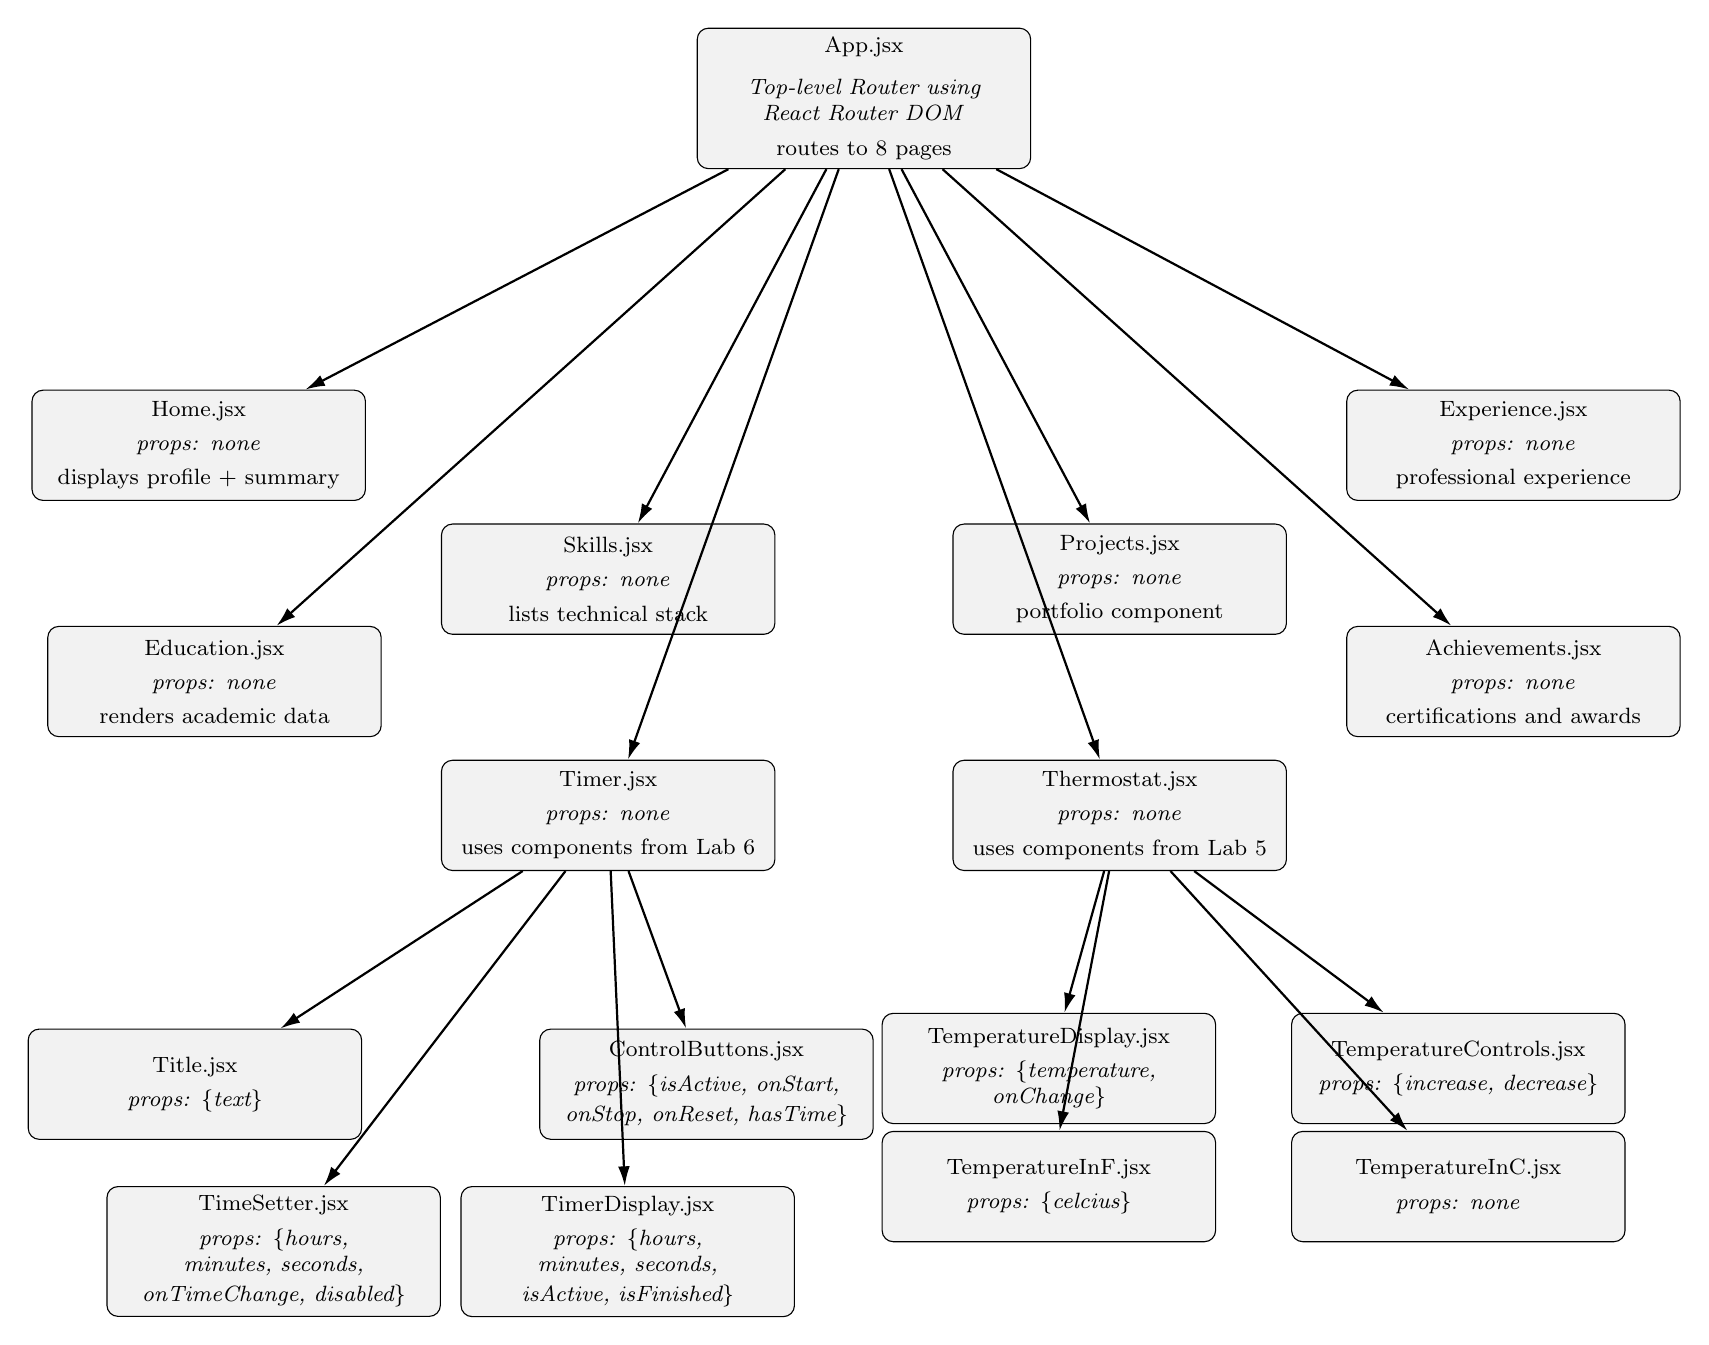
\begin{tikzpicture}[
    node distance=2cm and 2cm,
    every node/.style={
        draw,
        rounded corners,
        align=center,
        font=\footnotesize,
        fill=gray!10,
        text width=4cm,
        minimum height=1.4cm
    },
    arrow/.style={-{Latex[length=2.5mm,width=1.5mm]}, thick},
    prop/.style={font=\scriptsize, midway, fill=white, inner sep=1pt}
]

% Parent node 
\node (app) {App.jsx\\[0.2cm]
\textit{Top-level Router using React Router DOM}\\[0.1cm]
routes to 8 pages};

% Route components (fan layout) 
\node (home) [below left=2.8cm and 4.2cm of app] {Home.jsx\\[0.1cm]
\textit{props: none}\\[0.1cm]
displays profile + summary};

\node (education) [below left=5.8cm and 4cm of app] {Education.jsx\\[0.1cm]
\textit{props: none}\\[0.1cm]
renders academic data};

\node (skills) [below left=4.5cm and -1cm of app] {Skills.jsx\\[0.1cm]
\textit{props: none}\\[0.1cm]
lists technical stack};

\node (projects) [below right=4.5cm and -1cm of app] {Projects.jsx\\[0.1cm]
\textit{props: none}\\[0.1cm]
portfolio component};

\node (experience) [below right=2.8cm and 4cm of app] {Experience.jsx\\[0.1cm]
\textit{props: none}\\[0.1cm]
professional experience};

\node (achievements) [below right=5.8cm and 4cm of app] {Achievements.jsx\\[0.1cm]
\textit{props: none}\\[0.1cm]
certifications and awards};

\node (thermostat) [below right=7.5cm and -1cm of app] {Thermostat.jsx\\[0.1cm]
\textit{props: none}\\[0.1cm]
uses components from Lab 5};

\node (timer) [below left=7.5cm and -1cm of app] {Timer.jsx\\[0.1cm]
\textit{props: none}\\[0.1cm]
uses components from Lab 6};

% Arrows from App to each route 
\draw[arrow] (app) -- (home);
\draw[arrow] (app) -- (education);
\draw[arrow] (app) -- (skills);
\draw[arrow] (app) -- (projects);
\draw[arrow] (app) -- (experience);
\draw[arrow] (app) -- (achievements);
\draw[arrow] (app) -- (thermostat);
\draw[arrow] (app) -- (timer);

% Thermostat internal components (Lab 5) 
\node (tempdisplay) [below=1.8cm of thermostat,xshift=-0.9cm] {TemperatureDisplay.jsx\\[0.1cm]
\textit{props: \{temperature, onChange\}}};

\node (tempcontrols) [below=1.8cm of thermostat,xshift=4.3cm] {TemperatureControls.jsx\\[0.1cm]
\textit{props: \{increase, decrease\}}};

\node (tempinf) [below=3.3cm of thermostat,xshift=-0.9cm] {TemperatureInF.jsx\\[0.1cm]
\textit{props: \{celcius\}}};

\node (tempinc) [below=3.3cm of thermostat,xshift=4.3cm] {TemperatureInC.jsx\\[0.1cm]
\textit{props: none}};

\draw[arrow] (thermostat) -- (tempdisplay);
\draw[arrow] (thermostat) -- (tempcontrols);
\draw[arrow] (thermostat) -- (tempinf);
\draw[arrow] (thermostat) -- (tempinc);

% Timer internal components (Lab 6) 
\node (title) [below left=2cm and 1cm of timer] {Title.jsx\\[0.1cm]
\textit{props: \{text\}}};

\node (timesetter) [below left=4cm and 0cm of timer] {TimeSetter.jsx\\[0.1cm]
\textit{props: \{hours, minutes, seconds,}\\[0.05cm]
\textit{onTimeChange, disabled\}}};

\node (ctrlbtns) [below right=2cm and -3cm of timer] {ControlButtons.jsx\\[0.1cm]
\textit{props: \{isActive, onStart,}\\[0.05cm]
\textit{onStop, onReset, hasTime\}}};

\node (timerdisplay) [below right=4cm and -4cm of timer] {TimerDisplay.jsx\\[0.1cm]
\textit{props: \{hours, minutes, seconds,}\\[0.05cm]
\textit{isActive, isFinished\}}};

\draw[arrow] (timer) -- (title);
\draw[arrow] (timer) -- (timesetter);
\draw[arrow] (timer) -- (ctrlbtns);
\draw[arrow] (timer) -- (timerdisplay);

\end{tikzpicture}
\caption{Component Hierarchy — Lab 7: React Router Application (Routes + Nested Thermostat and Timer Components)}
\end{figure}


\subsection*{Rendered Output (Screenshot)}
\begin{figure}[H]
    \captionsetup{labelformat=empty}
    \centering
    \includegraphics[width=\textwidth]{Lab7/1.png}
    \caption{Screenshot 1: Home Page}
\end{figure}

\begin{figure}[H]
    \captionsetup{labelformat=empty}
    \centering
    \includegraphics[width=\textwidth]{Lab7/2.png}
    \caption{Screenshot 2: Education Page}
\end{figure}

\begin{figure}[H]
    \captionsetup{labelformat=empty}
    \centering
    \includegraphics[width=\textwidth]{Lab7/3.png}
    \caption{Screenshot 3: Skills Page}
\end{figure}

\begin{figure}[H]
    \captionsetup{labelformat=empty}
    \centering
    \includegraphics[width=\textwidth]{Lab7/4.png}
    \caption{Screenshot 4: Projects Page}
\end{figure}

\begin{figure}[H]
    \captionsetup{labelformat=empty}
    \centering
    \includegraphics[width=\textwidth]{Lab7/5.png}
    \caption{Screenshot 5: Experience Page}
\end{figure}


\begin{figure}[H]
    \captionsetup{labelformat=empty}
    \centering
    \includegraphics[width=\textwidth]{Lab7/6.png}
    \caption{Screenshot 6: Achievements Page}
\end{figure}

\begin{figure}[H]
    \captionsetup{labelformat=empty}
    \centering
    \includegraphics[width=\textwidth]{Lab7/7.png}
    \caption{Screenshot 7: Thermostat Page}
\end{figure}

\begin{figure}[H]
    \captionsetup{labelformat=empty}
    \centering
    \includegraphics[width=\textwidth]{Lab7/8.png}
    \caption{Screenshot 8: Timer Page Running}
\end{figure}

\begin{figure}[H]
    \captionsetup{labelformat=empty}
    \centering
    \includegraphics[width=\textwidth]{Lab7/9.png}
    \caption{Screenshot 9: Timer Page On Finish}
\end{figure}



\subsection*{Code Overview}

\subsubsection*{App.css}
\lstinputlisting[style=codestyle, language=CSS]{Lab7/App.css}

\subsubsection*{App.jsx (Router Setup)}
\lstinputlisting[style=codestyle, language=JavaScript]{Lab7/App.jsx}

\subsubsection*{CV Components}
\lstinputlisting[style=codestyle, language=JavaScript]{Lab7/components/Home.jsx}
\lstinputlisting[style=codestyle, language=JavaScript]{Lab7/components/Education.jsx}
\lstinputlisting[style=codestyle, language=JavaScript]{Lab7/components/Skills.jsx}
\lstinputlisting[style=codestyle, language=JavaScript]{Lab7/components/Projects.jsx}
\lstinputlisting[style=codestyle, language=JavaScript]{Lab7/components/Experience.jsx}
\lstinputlisting[style=codestyle, language=JavaScript]{Lab7/components/Achievements.jsx}

\subsubsection*{Thermostat Components (From Lab 5)}
\lstinputlisting[style=codestyle, language=JavaScript]{Lab7/components/Thermostat.jsx}
\lstinputlisting[style=codestyle, language=JavaScript]{Lab7/components/TemperatureDisplay.jsx}
\lstinputlisting[style=codestyle, language=JavaScript]{Lab7/components/TemperatureControls.jsx}
\lstinputlisting[style=codestyle, language=JavaScript]{Lab7/components/FahrenheitDisplay.jsx}
\lstinputlisting[style=codestyle, language=JavaScript]{Lab7/components/ConversionButton.jsx}

\subsubsection*{Timer Components (From Lab 6)}
\lstinputlisting[style=codestyle, language=JavaScript]{Lab7/components/Timer.jsx}
\lstinputlisting[style=codestyle, language=JavaScript]{Lab7/components/TimerDisplay.jsx}
\lstinputlisting[style=codestyle, language=JavaScript]{Lab7/components/TimeSetter.jsx}
\lstinputlisting[style=codestyle, language=JavaScript]{Lab7/components/ControlButtons.jsx}
\lstinputlisting[style=codestyle, language=JavaScript]{Lab7/components/Title.jsx}



\subsection*{Result}
A fully functional React application with eight distinct routes was successfully built using React Router v6.  
Each route loads a unique page component, and the overall app demonstrates:
\begin{itemize}
    \item Modular React component architecture.
    \item Routing integration across functional features.
    \item Hook-based state and effect management.
    \item Seamless composition of previous labs (Lab 5 + Lab 6) into new routes.
\end{itemize}



\subsection*{Conclusion}
This lab integrates multiple independent React modules into a single navigable application.  
It reinforces core React concepts such as routing, props, state management, and side-effect handling with \texttt{useEffect}.  
The project demonstrates scalable, modular front-end design suitable for full-stack deployment.

\subsection*{GitHub Repository}
The source code for all the labs can be found at the following GitHub repository:
\url{https://github.com/ashvp/Web-Technologies---Semester-5}
\newpage
\section*{Lab Exercise 8: Blog Dashboard using React Bootstrap}

\subsection*{Question}
Build a simple React application using React Bootstrap to create a blog dashboard with the following features:

\begin{itemize}
    \item A responsive \textbf{Navbar} (using React Bootstrap's \texttt{Navbar} component) with links to "Home" and "Posts".
    \item A grid of 3-4 \textbf{Blog Cards} (using Bootstrap's \texttt{Card}, \texttt{Row}, and \texttt{Col} components).
    \item Each card displays a post title, a short description, and a \texttt{Read More} button (using \texttt{Button} component).
    \item Use functional components and props to pass post data from parent to child components.
    \item Draw a component hierarchy diagram.
\end{itemize}



\subsection*{Design Description}
The application is built using React and React Bootstrap to create a clean, responsive blog dashboard UI.  
The dashboard includes:
\begin{itemize}
    \item A navigation bar at the top.
    \item A responsive grid layout for blog posts.
    \item Reusable blog card components that accept post data via props.
\end{itemize}

All components are built as functional components, with \texttt{props} used for communication between the parent (\texttt{App.jsx}) and child components (\texttt{BlogCard.jsx}).



\subsection*{Main Components and Props}

\begin{itemize}
    \item \textbf{App.jsx} - Root component that manages the overall structure and passes post data to the dashboard.
    \begin{itemize}
        \item \textit{Props:} None
        \item \textit{Responsibility:} Acts as parent container, imports all components, and defines post data as an array of objects.
    \end{itemize}

    \item \textbf{NavigationBar.jsx} - Displays the responsive navigation bar using React Bootstrap.
    \begin{itemize}
        \item \textit{Props:} \texttt{brandName}, \texttt{links} (array of link names or paths)
        \item \textit{Responsibility:} Provides top navigation with responsive collapse functionality.
    \end{itemize}

    \item \textbf{Dashboard.jsx} - Renders the grid layout of all blog posts.
    \begin{itemize}
        \item \textit{Props:} \texttt{posts} (array containing post title and description)
        \item \textit{Responsibility:} Uses Bootstrap’s grid system (\texttt{Row} and \texttt{Col}) to layout BlogCard components responsively.
    \end{itemize}

    \item \textbf{BlogCard.jsx} - A reusable card component displaying each post’s title, description, and “Read More” button.
    \begin{itemize}
        \item \textit{Props:} \texttt{title}, \texttt{description}
        \item \textit{Responsibility:} Displays data in a visually appealing Bootstrap card format.
    \end{itemize}
\end{itemize}



\subsection*{Component Hierarchy Diagram}
\begin{figure}[H]
\centering
% \hspace*{-1cm} % shift if cutting on right
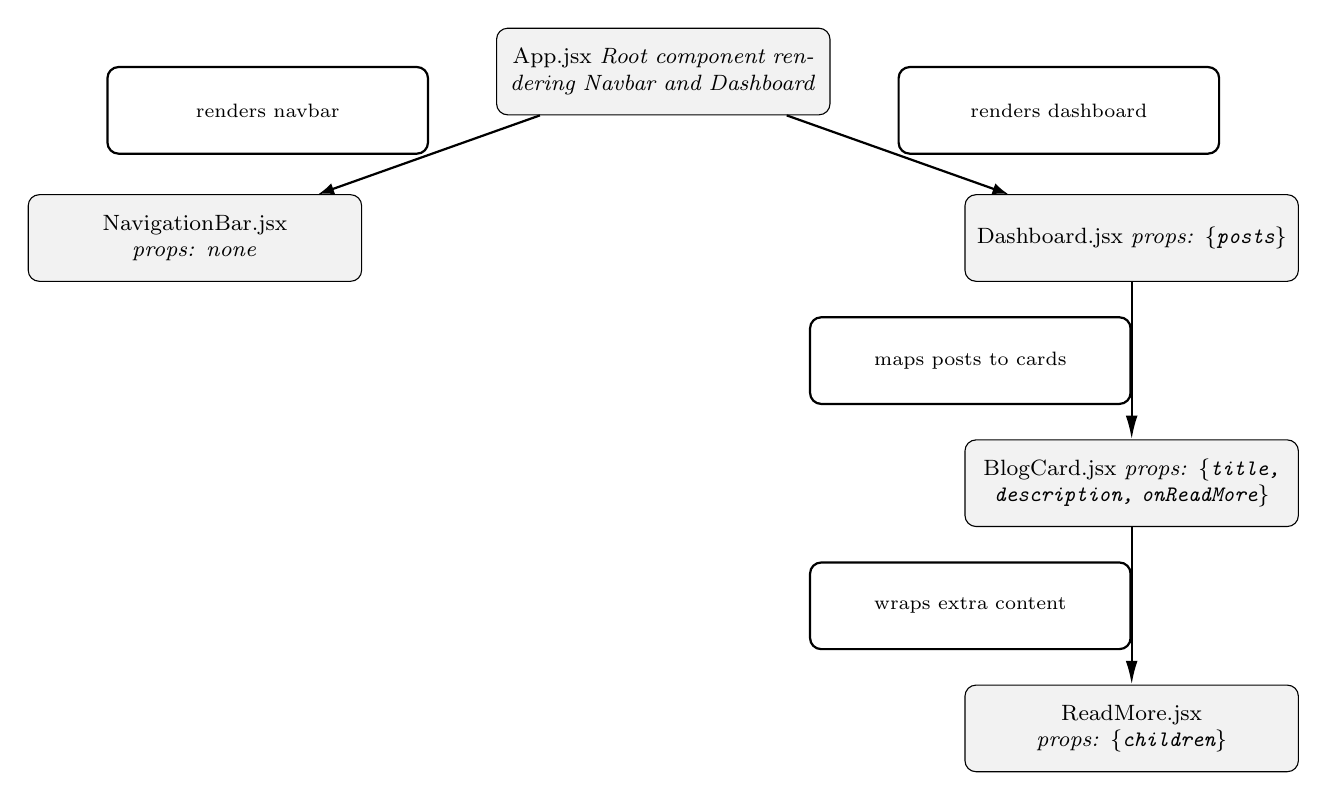
\begin{tikzpicture}[
  node distance=1cm and 1.5cm,
  every node/.style={
    draw,
    rounded corners,
    align=center,
    font=\footnotesize,
    fill=gray!10,
    text width=4cm,
    minimum height=1.1cm
  },
  level distance=1.4cm,
  edge from parent/.style={draw, thick, -{Latex[length=2mm,width=1.5mm]}},
  prop/.style={font=\scriptsize, midway, fill=white, inner sep=1pt}
]

% Root Node
\node (app) {App.jsx\
\textit{Root component rendering Navbar and Dashboard}};

% Children
\node (navbar) [below left=of app, xshift=-0.2cm] {NavigationBar.jsx\
\textit{props: none}};
\node (dashboard) [below right=of app, xshift=0.2cm] {Dashboard.jsx\
\textit{props: \texttt{\{posts\}}}};

% Nested under Dashboard
\node (blogcard) [below=2cm of dashboard] {BlogCard.jsx\
\textit{props: \texttt{\{title, description, onReadMore\}}}};
\node (readmore) [below=2cm of blogcard] {ReadMore.jsx\
\textit{props: \texttt{\{children\}}}};

% Arrows
\draw[-{Latex[length=2mm,width=1.5mm]}, thick] (app) -- node[prop,above left]{renders navbar} (navbar);
\draw[-{Latex[length=2mm,width=1.5mm]}, thick] (app) -- node[prop,above right]{renders dashboard} (dashboard);
\draw[-{Latex[length=3mm,width=1.5mm]}, thick] (dashboard) -- node[prop,left]{maps posts to cards} (blogcard);
\draw[-{Latex[length=3mm,width=1.5mm]}, thick] (blogcard) -- node[prop,left]{wraps extra content} (readmore);

\end{tikzpicture}
\caption{Component Hierarchy — Lab 8: Blog Dashboard (React + Bootstrap with Prop Flow)}
\end{figure}



\subsection*{Rendered Output (Screenshot)}
\begin{figure}[H]
    \captionsetup{labelformat=empty}
    \centering
    \includegraphics[width=\textwidth]{Lab8/1.png}
    \caption{Screenshot 1: Home Page}
\end{figure}

\begin{figure}[H]
    \captionsetup{labelformat=empty}
    \centering
    \includegraphics[width=\textwidth]{Lab8/2.png}
    \caption{Screenshot 2: Read More Button Clicked}
\end{figure}



\subsection*{Code Overview}

\subsubsection*{App.jsx}
\lstinputlisting[style=codestyle, language=JavaScript]{Lab8/App.jsx}

\subsubsection*{NavigationBar.jsx}
\lstinputlisting[style=codestyle, language=JavaScript]{Lab8/components/NavigationBar.jsx}

\subsubsection*{Dashboard.jsx}
\lstinputlisting[style=codestyle, language=JavaScript]{Lab8/components/Dashboard.jsx}

\subsubsection*{BlogCard.jsx}
\lstinputlisting[style=codestyle, language=JavaScript]{Lab8/components/BlogCard.jsx}



\subsection*{Result}
A fully functional, responsive React blog dashboard was successfully created using React Bootstrap.  
The Navbar and Cards adapt automatically to screen sizes, and component-level reusability was achieved through prop-driven data passing.



\subsection*{Conclusion}
This lab demonstrates practical usage of React Bootstrap components for building responsive, modular UIs.  
By combining props, grid layouts, and reusable components, the application achieves scalability, maintainability, and professional front-end design.

\subsection*{GitHub Repository}
The source code for all the labs can be found at the following GitHub repository:
\url{https://github.com/ashvp/Web-Technologies---Semester-5}
\newpage
\section*{Lab Exercise 9: Basic Blog Server using Node.js HTTP Module}

\subsection*{Question}
Build a simple Node.js blog server using only the built-in \texttt{http} module by creating a \texttt{server.js} file. Implement basic routing as follows:

\begin{itemize}
    \item A \textbf{GET endpoint} at \texttt{/} that returns an HTML home page with inline navigation links to “Home” (\texttt{/}) and “Posts” (\texttt{/posts}).
    \item A \textbf{GET endpoint} at \texttt{/posts} that dynamically generates an HTML page displaying 3-4 blog posts (titles and descriptions) from a hardcoded array using a loop.
    \item A \textbf{404 handler} for unmatched routes, returning a styled HTML error message.
\end{itemize}



\subsection*{Design Description}
This lab demonstrates the creation of a minimal web server in Node.js without using external frameworks like Express.  
The server handles routing manually using conditional logic on the request URL, serving different pages based on the endpoint.

The implementation includes:
\begin{itemize}
    \item \textbf{Home Page:} Static HTML file with navigation links to other routes.
    \item \textbf{Posts Page:} Dynamically generated HTML content using a hardcoded JavaScript array of post objects.
    \item \textbf{Error Handling:} Custom 404 response for undefined routes.
\end{itemize}



\subsection*{Main Files and Their Roles}

\begin{itemize}
    \item \textbf{server.js} - Entry point of the Node application. Creates an HTTP server, handles routing logic, and serves content.
    \item \textbf{components/homePage.html} - Static home page served at the root endpoint (\texttt{/}).
    \item \textbf{components/blog.html} - Template HTML structure used to render blog posts dynamically.
    \item \textbf{components/error.html} - HTML error page returned for invalid routes.
    \item \textbf{data/BlogPosts.js} - Exports a hardcoded array of blog post objects, each containing \texttt{title} and \texttt{description}.
    \item \textbf{routes/home.js} - Handles logic for rendering and returning the home page.
    \item \textbf{routes/posts.js} - Handles logic for looping through the post data and generating the blog page.
    \item \textbf{routes/error.js} - Exports a function to handle 404 errors gracefully.
\end{itemize}



% \subsection*{Component Hierarchy Diagram}
% \begin{center}
% \includegraphics[width=0.85\textwidth]{Lab9/images/hierarchy.png}
% \end{center}



\subsection*{Rendered Output (Screenshots)}
\begin{figure}[H]
    \captionsetup{labelformat=empty}
    \centering
    \includegraphics[width=\textwidth]{Lab9/1.png}
    \caption{Screenshot 1: Home Page}
\end{figure}

\begin{figure}[H]
    \captionsetup{labelformat=empty}
    \centering
    \includegraphics[width=\textwidth]{Lab9/2.png}
    \caption{Screenshot 2: Posts Page with Dynamic Blog Posts}
\end{figure}

\begin{figure}[H]
    \captionsetup{labelformat=empty}
    \centering
    \includegraphics[width=\textwidth]{Lab9/3.png}
    \caption{Screenshot 3: Custom 404 Error Page - Invalid Route}
\end{figure}

\subsection*{Code Overview}

\subsubsection*{server.js}
\lstinputlisting[style=codestyle, language=JavaScript]{Lab9/server.js}

\subsubsection*{routes/home.js}
\lstinputlisting[style=codestyle, language=JavaScript]{Lab9/routes/home.js}

\subsubsection*{routes/posts.js}
\lstinputlisting[style=codestyle, language=JavaScript]{Lab9/routes/posts.js}

\subsubsection*{routes/error.js}
\lstinputlisting[style=codestyle, language=JavaScript]{Lab9/routes/error.js}

\subsubsection*{data/BlogPosts.js}
\lstinputlisting[style=codestyle, language=JavaScript]{Lab9/data/BlogPosts.js}

\subsubsection*{components/homePage.html}
\lstinputlisting[style=codestyle, language=HTML]
{Lab9/components/homePage.html}

\subsubsection*{components/blog.html}
\lstinputlisting[style=codestyle, language=HTML]{Lab9/components/blog.html}

\subsubsection*{components/error.html}
\lstinputlisting[style=codestyle, language=HTML]{Lab9/components/error.html}



\subsection*{Result}
The Node.js HTTP server was successfully implemented with basic routing and dynamic content generation.  
Navigating to \texttt{http://localhost:3000/} renders the home page, while \texttt{/posts} dynamically displays 3-4 blog posts from the array.  
Invalid routes correctly return a custom 404 page.



\subsection*{Conclusion}
This lab demonstrates how to create a functional web server using only Node.js’ built-in \texttt{http} and \texttt{fs} modules.  
It showcases:
\begin{itemize}
    \item Manual routing without frameworks.
    \item Dynamic HTML generation using JavaScript loops.
    \item Modular separation of route handlers and data sources.
\end{itemize}
The project lays the foundation for understanding core Node.js web concepts before introducing Express.js in advanced labs.

\newpage
\section*{Lab Exercise 10: Node.js HTTP Server with URL Routing and Logging}

\subsection*{Question}
Create an HTTP server using Node.js. Use the \texttt{url} module to parse the incoming request URL and extract the pathname for routing decisions.

\begin{itemize}
    \item For pathname \texttt{/}, read and serve the content of \texttt{index.html}. If the file doesn't exist, log an error in a log file but still return a basic “Home Page” message.
    \item For pathname \texttt{/about}, read and serve the content of \texttt{about.html} similarly, logging an error if the file is missing.
    \item For any other pathname, return a 404 status with “Page Not Found”.
    \item Create two simple HTML files — \texttt{index.html} and \texttt{about.html} — with a title and a short paragraph.
    \item Implement logging of server events and errors into a text file named \texttt{Logs.txt}.
    \item Test the server locally.
\end{itemize}



\subsection*{Design Description}
This lab focuses on building a simple Node.js server without frameworks, utilizing the \texttt{http}, \texttt{fs}, and \texttt{url} modules to serve HTML pages based on URL routes.  
The design demonstrates:
\begin{itemize}
    \item Manual routing logic for multiple paths.
    \item Error handling when files are missing.
    \item Logging of both successful and failed requests.
\end{itemize}

The program reads static HTML files from the local \texttt{components/} directory and sends them as responses, while also maintaining logs in a text file for traceability.



\subsection*{Main Files and Their Responsibilities}

\begin{itemize}
    \item \textbf{server.js} - Entry point that creates the HTTP server, parses URL paths, routes requests, and delegates to route handlers.
    \item \textbf{routes/home.js} - Handles requests to the root path (\texttt{/}); serves \texttt{home.html}.
    \item \textbf{routes/about.js} - Handles requests to the \texttt{/about} path; serves \texttt{about.html}.
    \item \textbf{components/home.html} - HTML file for the home page, containing a title and a paragraph.
    \item \textbf{components/about.html} - HTML file for the about page, containing a title and a paragraph.
    \item \textbf{utils/logger.js} - Contains helper functions to log request details and errors to \texttt{Logs.txt}.
    \item \textbf{Logs.txt} - Log file that records request events, timestamps, and error messages.
\end{itemize}



% \subsection*{Component Hierarchy Diagram}
% \begin{center}
% \includegraphics[width=0.85\textwidth]{Lab10/images/hierarchy.png}
% \end{center}



\subsection*{Rendered Output (Screenshots)}
\begin{figure}[H]
    \captionsetup{labelformat=empty}
    \centering
    \includegraphics[width=\textwidth]{Lab10/1.png}
    \caption{Screenshot 1: Home Page served successfully.}
\end{figure}

\begin{figure}[H]
    \captionsetup{labelformat=empty}
    \centering
    \includegraphics[width=\textwidth]{Lab10/2.png}
    \caption{Screenshot 2: About Page Rendered Successfully.}
\end{figure}

\begin{figure}[H]
    \captionsetup{labelformat=empty}
    \centering
    \includegraphics[width=\textwidth]{Lab10/3.png}
    \caption{Screenshot 3: Custom 404 Page Not Found response for invalid routes.}
\end{figure}

\begin{figure}[H]
    \captionsetup{labelformat=empty}
    \centering
    \includegraphics[width=\textwidth]{Lab10/4.png}
    \caption{Screenshot 4: Internal Server Error logged when abot.html is missing.}
\end{figure}



\subsection*{Code Overview}

\subsubsection*{server.js}
\lstinputlisting[style=codestyle, language=JavaScript]{Lab10/server.js}

\subsubsection*{routes/home.js}
\lstinputlisting[style=codestyle, language=JavaScript]{Lab10/routes/home.js}

\subsubsection*{routes/about.js}
\lstinputlisting[style=codestyle, language=JavaScript]{Lab10/routes/about.js}

\subsubsection*{utils/logger.js}
\lstinputlisting[style=codestyle, language=JavaScript]{Lab10/utils/logger.js}

\subsubsection*{HTML Files}
\lstinputlisting[style=codestyle, language=HTML]{Lab10/components/home.html}
\lstinputlisting[style=codestyle, language=HTML]{Lab10/components/about.html}

\subsubsection*{Logs.txt (Sample Output)}
\lstinputlisting[style=codestyle]{Lab10/Logs.txt}



\subsection*{Result}
The HTTP server successfully handles multiple routes:
\begin{itemize}
    \item Accessing \texttt{http://localhost:3000/} serves the home page.
    \item Accessing \texttt{http://localhost:3000/about} serves the about page.
    \item Accessing any other URL returns a custom 404 response.
\end{itemize}

If any HTML file is missing, the server logs an appropriate error in \texttt{Logs.txt} while still responding with a fallback message to ensure reliability.



\subsection*{Conclusion}
This lab effectively demonstrates:
\begin{itemize}
    \item Routing control in Node.js using the \texttt{url} module.
    \item File reading and serving via the \texttt{fs} module.
    \item Error handling and event logging through a custom utility.
\end{itemize}

It provides a foundational understanding of low-level HTTP server mechanics before transitioning to frameworks like Express.js.


\end{document}
